\begin{frame}
\frametitle{Скорость CPU, памяти и дисков}
\begin{itemize}
  \item Некоторое время назад (80-90-ые года) скорость CPU росла довольно быстро
  \begin{itemize}
    \item вместе со скоростью CPU росли объемы оперативной памяти и дисков.
  \end{itemize}
  \item Однако скорость оперативной памяти и дисков не успевала за ростом:
  \begin{itemize}
    \item разрыв между скоростью памяти и CPU так или иначе заполняется кешами;
    \item но между оперативной памятью и дисками просто пропасть.
  \end{itemize}
\end{itemize}
\end{frame}

\begin{frame}
\frametitle{Массивы независимых (недорогих) дисков}
\begin{itemize}
  \item RAID (Redundant Array of Independent (Inexpenisve) Disks) - объединение
  из нескольких физических устройств в одно логические устройство:
  \begin{itemize}
    \item несколько дисков позволяют достигать большего объема;
    \item при дублировании данных на несколько дисков мы можем читать данные с
    любого из них - несколько параллельных запросов повышают производительность;
    \item имея копии данных мы можем переживать поломки дисков/порчу данных.
  \end{itemize}
\end{itemize}
\end{frame}

\begin{frame}
\frametitle{Redundancy is important}
\begin{itemize}
  \item В спецификации дисков зачастую указывают параметры MTTF/MBTF/AFR:
  \begin{itemize}
    \item MTTF (Mean Time to Failure) - для SSD где-то в районе 2 млн. часов;
    \item для массива из 1000 одинаковых дисков получим что-то вроде 2000
    часов;
    \item чем больше независмых устройств - тем больше вроятность отказа
    системы.
  \end{itemize}
  \item Для массива из дисков полезен еще дополнительный параметр MTTR:
  \begin{itemize}
    \item MTTR (Mean Time To Repair) - время необходимое на обнаружения сбоя
    диска, его замену и восстановление данных на нем;
    \item никакой RAID вас не спасет, если вам нужно 100500 лет чтобы заменить
    плохой диск.
  \end{itemize}
\end{itemize}
\end{frame}

\begin{frame}
\frametitle{RAID 1}
\framesubtitle{Mirroring}
\begin{itemize}
  \item Самый очевидный способ повысить надежность - простое дублирование:
  \begin{itemize}
    \item вы просто пишите каждую порцию данных на 2 (N) дисков параллельно;
    \item при таком подходе можно переживать 1 (N-1) отказ диска.
  \end{itemize}
  \item Минусы:
  \begin{itemize}
    \item требуется в 2 (N) раза больше пространства;
    \item "хвосты" - запись со скоростью самого медленного диска.
  \end{itemize}
  \item Плюсы:
  \begin{itemize}
    \item чтение в 2 (N) раза быстрее - любая порция данных может быть прочитана
    с любого из дисков (если он в строю);
    \item т. е. мы можем обрабатывать несколько запросов на чтение параллельно.
  \end{itemize}
\end{itemize}
\end{frame}

\begin{frame}
\frametitle{RAID 2}
\framesubtitle{Parity}
\begin{center}
  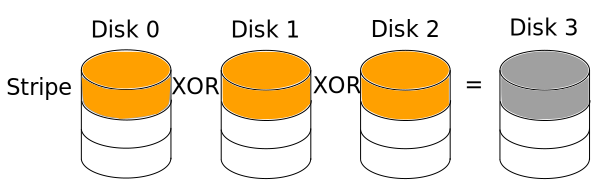
\includegraphics[width=.8\linewidth]{parity.png}
\end{center}
\begin{itemize}
  \item Вместо полного дублирования мы можем использовать проверку четности:
  \begin{itemize}
    \item пусть у нас будет N дисков с данными - на каждый из них пишется своя
    порция информации;
    \item добавим к ним еще один диск - диск четности;
    \item диск четности хранит XOR соответствующих бит дисков с данными;
  \end{itemize}
\end{itemize}
\end{frame}

\begin{frame}
\frametitle{RAID 2}
\framesubtitle{Matrix Form}
\[
  \left(
    \begin{array}{cccc}
      1 & 1 & 1 & 1
    \end{array}
  \right) \times \left(
    \begin{array}{c}
      d_0 \\
      d_1 \\
      d_2 \\
      d_3
    \end{array}
  \right) = 0
\]
\begin{itemize}
  \item Мы можем записать условие четности в матричном виде:
  \begin{itemize}
    \item сложение - XOR;
    \item умножение - AND;
    \item т. е. XOR всех бит данных с битом четности должен давать 0.
  \end{itemize}
\end{itemize}
\end{frame}

\begin{frame}
\frametitle{RAID 2}
\framesubtitle{Generalized Parity}
\[
  \left(
    \begin{array}{ccccccc}
      1 & 0 & 1 & 0 & 1 & 0 & 1 \\
      0 & 1 & 1 & 0 & 0 & 1 & 1 \\
      0 & 0 & 0 & 1 & 1 & 1 & 1
    \end{array}
  \right) \times \left(
    \begin{array}{c}
      d_0 \\
      d_1 \\
      d_2 \\
      d_3 \\
      d_4 \\
      d_5 \\
      d_6
    \end{array}
  \right) = \left(
    \begin{array}{c}
      0 \\
      0 \\
      0
    \end{array}
  \right)
\]
\begin{itemize}
  \item Мы можем проверять четность для некоторого подмножества бит
  \begin{itemize}
    \item если каждый диск входит хотя бы в одно подмножество;
    \item и для каждой пары дисков есть подмножество, в которое входит только
    один из них;
    \item то мы легко можем исправлять сразу две ошибки.
  \end{itemize}
\end{itemize}
\end{frame}

\begin{frame}
\frametitle{RAID 2}
\begin{itemize}
  \item В общем случае нужную систему уравнений нам дают коды Хэмминга:
  \begin{itemize}
    \item для $C$ дисков с битами четности можно использовать до $2^C - 1 - C$
    дисков с данными;
    \item т. е. всего $2^C - 1$ дисков;
    \item и переживать потерю любых двух дисков.
  \end{itemize}
  \item Недостатки:
  \begin{itemize}
    \item нужно сравнительно много дисков, чтобы получить какой-то выигрыш по
    сравнению с RAID 1 нужно как минимум 7 дисков;
    \item запись происходит со скоростью самого медленного диска.
  \end{itemize}
  \item Достоинства:
  \begin{itemize}
    \item дополнительные расходы дискового пространства уменьшаются
    экспоненциально.
  \end{itemize}
\end{itemize}
\end{frame}
